%----------------------------------------------------------------------------------------
%	SECTION 1.1
%----------------------------------------------------------------------------------------

\section{Quotient Groups.}
\label{section1}

\begin{definition}
    Let $G$ and $H$ be groups and let $\phi:G \rightarrow H$ be a homomorphism
    of $G$ into  $H$. We define the \textbf{fiber} of $\phi$ over an element $h
    \in H$ to be the preimage of  $h$ under  $\phi$, i.e.  $\inv{\phi}(h)=\{g
    \in G : \phi(g)=h\}$.
\end{definition}

\begin{figure}[h]
    \centering
    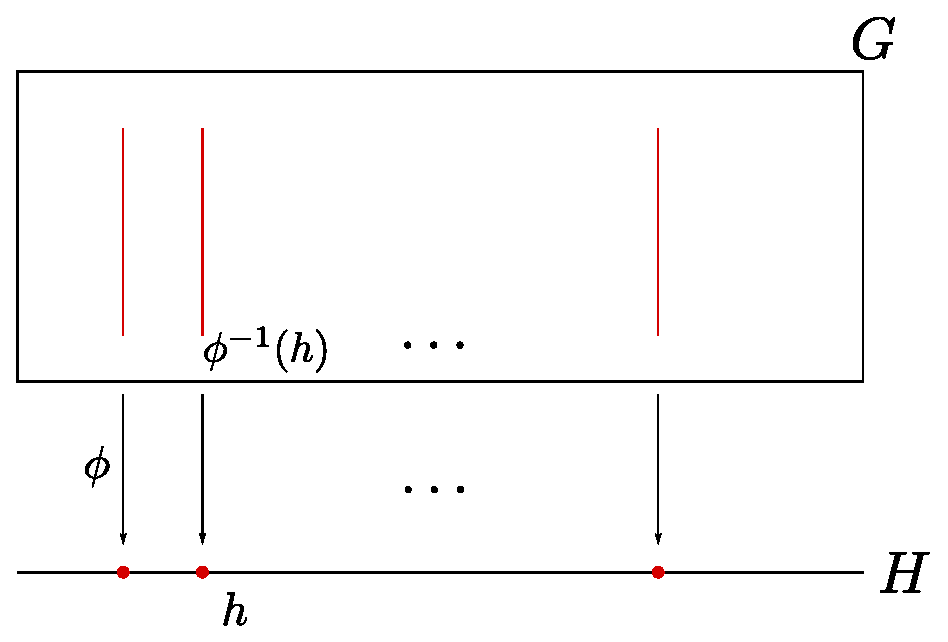
\includegraphics[scale = 0.5]{Figures/Chapter3/fibers.eps}
    \caption{The fibers of the elements of $H$ represented as vertical lines.}
    \label{fig_3.1}
\end{figure}

We can immediately define a special fiber for any homomorphisms.

\begin{definition}
    Let $G$ and  $H$ be groups and let  $\phi:G \rightarrow H$ be a homomorphism
    of $G$ into  $H$. We define the \textbf{kernel} of $\phi$ to be the fiber
    $\inv{\phi}(e')$ where $e'$ is the identity of  $H$. That is:
    \begin{equation}
        \ker{\phi}=\{g \in G : \phi(g)=e'\}
    \end{equation}
\end{definition}

\begin{lemma}\label{3.1.1}
    $\phi:G \rightarrow H$ is a $1-1$ homomorphism if and only if
    $\ker{\phi}=\vbrack{e}$.
\end{lemma}
\begin{proof}
    We have that $\phi(e)=e'$, thus since $\phi$ is $1-1$, we have $\phi(a)=e'$
    implies $a=e$.

    On the other hand, suppose $\ker{\phi}=\vbrack{e}$, and that
    $\phi(a)=\phi(b)$. Then $\phi(a)\inv{\phi(b)}=\phi(a\inv{b})=e'$, so that
    $a\inv{b}=e$. That is, $a=b$.
\end{proof}

\begin{lemma}\label{3.1.2}
    Let $G$ and  $H$ be groups and let  $\phi:G \rightarrow H$ be a homomorphism
    of $G$ into  $H$. Then $\ker{\phi} \leq G$, and $\phi(G) \leq H$.
\end{lemma}
\begin{proof}
    We have that $\phi(e)=e'$ and for any $a,b \in \ker{\phi}$, that
    $\phi(ab)=\phi(a)\phi(b)=e'$, and that $\phi(\inv{a})=\inv{\phi(a)}=e'$.
    This makes $e',ab, \inv{a} \in \ker{\phi}$.
\end{proof}

\begin{example}\label{3.1}
    Let $Z_n=\vbrack{x}$ be the cyclic group of order $n$ and define the
    homomorphism  $\phi:\Z \rightarrow Z_n$ by $a \rightarrow x^a$. Then
    $\phi(a+b)=x^{a+b}=a^ax^b=\phi(a)\phi(b)$, so $\phi$ is a homomrphsim.
    Moreover,  $\inv{\phi}(x^a)=\{m \in \Z : m \equiv a \mod{n}\}=n\Z$. So the
    set of fibers is $\faktor{\Z}{n\Z}$, moreover, we get the kernel of $\phi$
    to be  $\ker{\phi}=\{m \in \Z : m \equiv 0 \mod{n}\}=n\Z$ the set of all
    multiples of $n$.
\end{example}

This motivates the following results.

\begin{theorem}\label{3.1.3}
    Let $\inv{\phi}(H)$ be the set of all fibers of $\phi$ under elements of
    $H$, and define the operation $\inv{\phi}(a)\inv{\phi}(b)=\inv{\phi}(ab)$.
    Then $\inv{\phi}(H)$ forms a group under this operation.
\end{theorem}
\begin{proof}
    Let $\inv{\phi}(a)$ and $\inv{\phi}(b)$ be fibers of  $\phi$ under  $a$ and
     $b$ re spectively. Then for $g \in \inv{\phi}(a)$ and  $g' \in
     \inv{\phi}(b)$, we have  $\phi(gg')=\phi(g)\phi(g')=ab$, so that $gg' \in
     \inv{\phi}(ab)$, so this ensures that the operation is well defined.
     Moreover, we have that $\inv{\phi}(H)$ satisfies associativity because of
     the associativity of  $H$.

     Notice, then that  $\inv{\phi}(e)$ is the identity, as, for $g_e \in
     \inv{\phi}(e)$, $\phi(gg_e)=\phi(g)\phi(g_e)=ae=a=ea=\phi(g_e)\phi(g)=
     \phi(g_eg)$, where $g \in \inv{\phi}(a)$ and $g_e \in \inv{\phi}(e)$.
     Similarly, we find that $\inv{\phi}(\inv{a})$ is the inverse of $\inv{\phi}(a)$
     of $\inv{\phi}(H)$.
\end{proof}

\begin{definition}
    Let $G$ and  $H$ be groups, and let  $\phi:G \rightarrow H$ be a homomorphsm
    with $\ker{\phi}=K$. We deine the \textbf{quotient group} of $G$
    \textbf{mod} $K$ to be the group $\faktor{G}{K}$ of all fibers of $\phi$
    under elements of $K$.
\end{definition}

\begin{lemma}\label{3.1.4}
    Let $\phi$ be a homomorphism defined on a group  $G$ with  $\ker{\phi}=K$.
    Then for any fiber $\inv{\phi(a)} \in \faktor{G}{K}$, $a \in K$. we have
    for any $u \in \inv{\phi}(a)$, that $\inv{\phi}(a)=\{uk : k \in K\}$ and
    $\inv{\phi}(a)=\{ku : k \in K\}$.
\end{lemma}
\begin{proof}
    Let $uK=\{uk : k \in K\}$. Then since $\phi(u)=a$, for any $k \in K$, we
    have  $\phi(uk)=\phi(u)\phi(k)=ae=a$, making $uk \in \inv {\phi}(a)$. On the
    other hand, for some other $x \in \inv{\phi}(a)$, let $k=\inv{u}x$. Then
     $\phi(k)=\phi(\inv{u})\phi(x)=\inv{\phi(u)}\phi(x)=\inv{a}a=e'$, so $k \in
     K$. Then  $x=uk$, this  $x \in uK$. This makes  $\inv{\phi}(a)=uK$. The
     second assertion follows similarly.
\end{proof}

\begin{definition}
    Let $G$ be a group, and let  $H \leq G$. For any  $g \n G$, we define the
     \textbf{left} and \textbf{right cosets} of $H$ in $G$ to be the sets
     $gH=\{gh : h \in h\}$ and $Hg=\{hg : h \in h\}$, respectively.
\end{definition}

\begin{lemma}\label{3.1.5}
    Let $G$ and  $H$ be groups and  $\phi:G \rightarrow H$ a homomorphism with
    kernel $K$. Then for any  $g \in G$,  $gK=Kg$.
\end{lemma}
\begin{proof}
    By the previous lemma \ref{3.1.4}, if $a \in gK$ then  $a \in \inv{\phi}(g)$,
    which makes $a=kg$ for some  $k \in K$, thus  $a \in Kg$. Similarly, if  $b
    \in Kg$, then  $b \in gK$.
\end{proof}

It is much easier to think in terms of cosets, rather than fibers, so we develop
the theory of cosets furthur. In particucular, if $G$ is a group, and  $K$ is
the kernel of some homomorphism  $\phi$ defined on  $G$, then define the
operation of  \textbf{coset multiplication} by the rule $aKbK=abK$. Then we get
the following result.

\begin{theorem}\label{3.1.6}
    Let $G$ be a group and  $\phi$ a homomorphism on $G$ with kernel  $K$. Then
    the set of all cosets of  $K$ in  $G$ forms a group under coset
    multiplication.
\end{theorem}
\begin{proof}
    Let $a' \in aK$ and  $b' \in bK$. Then  $a'=ak_1$ and $b'=bk_2$, thus
    $a'b'=(ak_1)(bk_2)=a(k_1b)k_2=a(bk')k_2=ab(k'k_2)=abk''$. This makes $a'b'
    \in abK$, and by definition  $aKbK=abK$, we get  $a'b'K=abK$. Therefore
    coset multiplication is well defined.

    Now, notice that for the identity element  $e \in G$, that $eK=K$ satisfies
    $aKK=KaK=aeK=aK$. Moreover, for the inverse  $\inv{a} \in G$ of $a$, we have
     $\inv{a}KaK=aK\inv{a}K=a\inv{a}K=eK=K$. So $K$ is the identity element and
     $\inv{a}K$ is the inverse of  $aK$. Lastly, associativity is inherited from
     the associativity of $G$; i.e.
     $(aKbK)cK=abKcK=(ab)cK=a(bc)K=aKbcK=aK(bKcK)$
\end{proof}
\begin{corollary}
    The group of cosets of $K$ in  $G$ is precisely the quotient group
    $\faktor{G}{K}$.
\end{corollary}
\begin{proof}
    This follows directly from lemma \ref{3.1.4}. Since $\faktor{G}{K}$ is the
    set of all fiber $\inv{\phi}(a)$ Then notice that $\inv{\phi}(a)=aK=Ka$.
\end{proof}

\begin{example}\label{3.2}
    \begin{enumerate}
        \item[(1)] For $\Z$ and  $Z_n=\vbrack{x}$ in example \ref {3.2}, the
            homomorphism $\phi:a \rightarrow x^a$ has kernel $n\Z$, so the
            cosets of  $n\Z$ in  $\Z$ are of the form  $a+n\Z$ which are the
            elements $\mod{n}$. Thus the quotient group is $\faktor{\Z}{n\Z}$.

        \item[(2)] Let $G$ and  $H$ be isomorphic to each other via the
            isomorpism  $\phi:G \rightarrow H$. Then $\ker{\phi}=\vbrack{e}$,
            and so the cosets are all $a\vbrack{e}=a$ so we get
            $\faktor{G}{\vbrack{e}}=G$.

        \item[(3)] Let $G$ be a group and define  $\phi:G \rightarrow
            \vbrack{e}$ by $g \rightarrow e$. Then $\phi$ is a homomorphism with
             kernel $\ker{\phi}=G$. The cosets are precisely all $gG=G$.Thus
             the quotient group is $\faktor{G}{G} \simeq \vbrack{e}$

         \item[(4)] Define the map $\phi:\R^2 \rightarrow \R$ to be the
             pojection onto the $x$-axis $(x,y) \rightarrow x$. Then
             $\phi((x_1,y_1)+(x_2,y_2))=x_1+x_2=\phi((x_1,y)+(x_2,y'))$. So
             $\phi$ is a homomorphism. Then $\ker{\phi}=\{x \in \R :
             \phi(x,y)=0\}=(0,\R)$; i.e. the $y$-axis. Then the cosets are all
             the vertical lines $(x,\R)$, of the quotient group
             $\faktor{\R^2}{(0,\R)}$. Taking $(x,\R) \rightarrow x$, we get
             $\faktor{\R^2}{(0,\R)} \simeq \R$.

         \item[(5)] Consider the quaternions $\Hb$ and the Kelin-$4$ group  $V_4$.
             Take  $\phi:\Hb \rightarrow V_4$ defined by the rule $\pm 1
             \rightarrow 1$, $\pm i \rightarrow a$, $\pm j \rightarrow b$, and
              $\pm k \rightarrow c$. Then  $\phi$ is a homomorphism with kernel
               $\ker{\phi}=\vbrack{-1,1}$. Then the cosets of the quotient group
                $\faktor{\Hb}{\vbrack{-1,1}}$ are all $\vbrack{-1,1}$,
                $\vbrack{-i,i}$, $\vbrack{-j,j}$, and $\vbrack{-k,k}$, all
                collaped to  $1,a,b,c \in V_4$.
    \end{enumerate}
\end{example}
